\documentclass[12pt]{article}
\usepackage{fancyhdr}     % Enhanced control over headers and footers 
\usepackage[T1]{fontenc}  % Font encoding
\usepackage{mathptmx}     % Choose Times font 
\usepackage{microtype}    % Improves line breaks      
\usepackage{setspace}     % Makes the document look like horse manure 
\usepackage{lipsum}       % For dummy text
\usepackage{graphicx, xcolor}
\usepackage{caption}
\usepackage{subcaption}
\pagestyle{fancy} % Default page style 
\lhead{Yuhang Jiang, CSE152A, Professor Manmohan}
\chead{}
\rhead{\thepage}
\lfoot{}
\cfoot{}
\rfoot{}
\usepackage{hyperref}
\renewcommand{\headrulewidth}{1pt}
\renewcommand{\footrulewidth}{0pt}
\setlength{\parindent}{20pt}
\usepackage{etoolbox}
\AtBeginEnvironment{quote}{\par\singlespacing\small}
\usepackage[superscript,biblabel]{cite}
\usepackage[super,sort]{natbib}
\makeatletter \renewcommand{\@citess}[1]{\textsuperscript{\,[#1]}} \makeatother
\RequirePackage{filecontents}
\setcitestyle{square}
\setlength\headheight{0pt} %Slight increase to header size
\graphicspath{{./}}
\begin{filecontents}{reference.bib}
	@article{fifa, author = "fifa", title="111", year=3001}
	@article{ucl, author = "BBB", title="222", year=3002}
	@article{ccc, author = "CCC", title="333", year=3003}
\end{filecontents}

\begin{document}
	\begin{center}
		\begin{tabular}{c}
			\textbf{Computer Vision Self-Study: Semi-automated offside technology} \\
		\end{tabular}
	\end{center}
	
	\section{Introduction}
		\indent In football matches, the referee's penalty for offside has always been a difficult problem. Since 2018, Video Assistant Referee (VAR) has been officially written into the law of football, some potential offsides and fouls will be watched by the Video Assistant Referee behind the scenes to alert the referee. This greatly improves the accuracy of the penalty, but it also slows down the pace of the game.
		
		The just-concluded FIFA World Cup Qatar 2022 used a Semi-automated offside technology(SAOT) for the first time.
		\begin{quote}
			"The new technology uses 12 dedicated tracking cameras mounted underneath the roof of the stadium to track the ball and up to 29 data points of each individual player, 50 times per second, calculating their exact position on the pitch. The 29 collected data points include all limbs and extremities that are relevant for making offside calls."\cite{fifa}
		\end{quote}

	\begin{figure}[ht!]
		\centering
		\begin{subfigure}[b]{0.35\textwidth}
			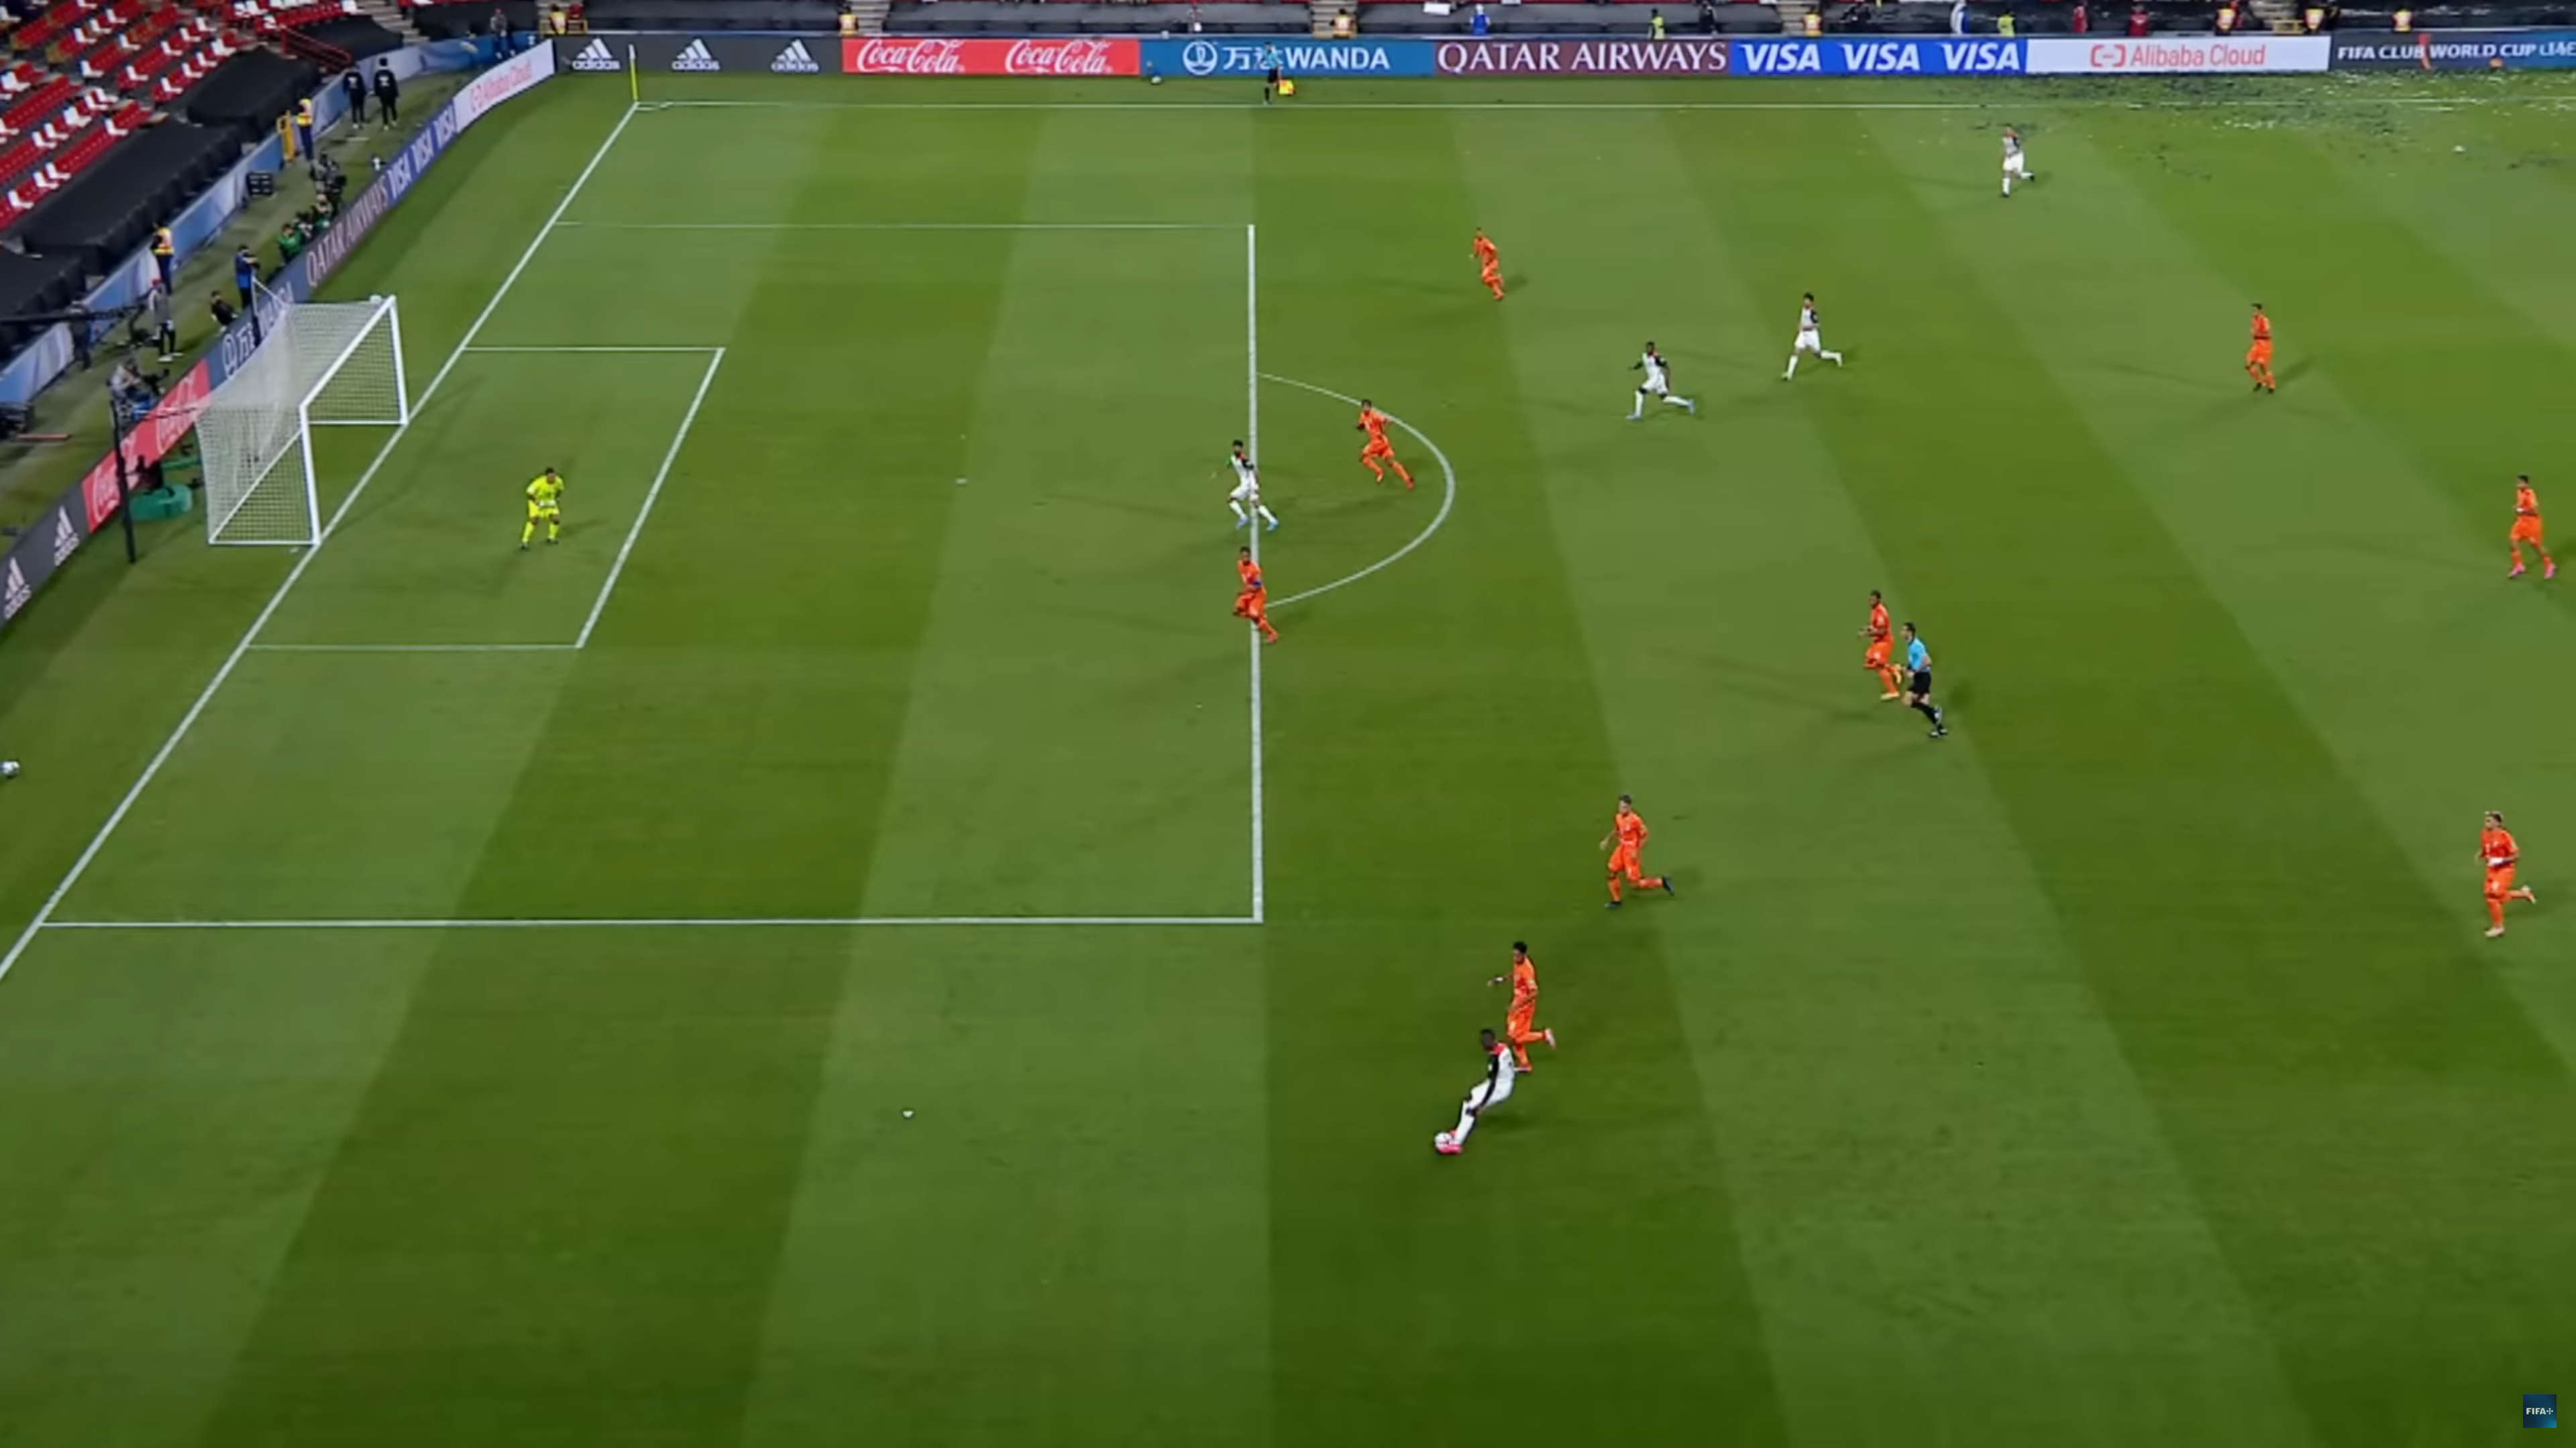
\includegraphics[width=\textwidth]{pic2.png}
		\end{subfigure}
		\begin{subfigure}[b]{0.35\textwidth}
			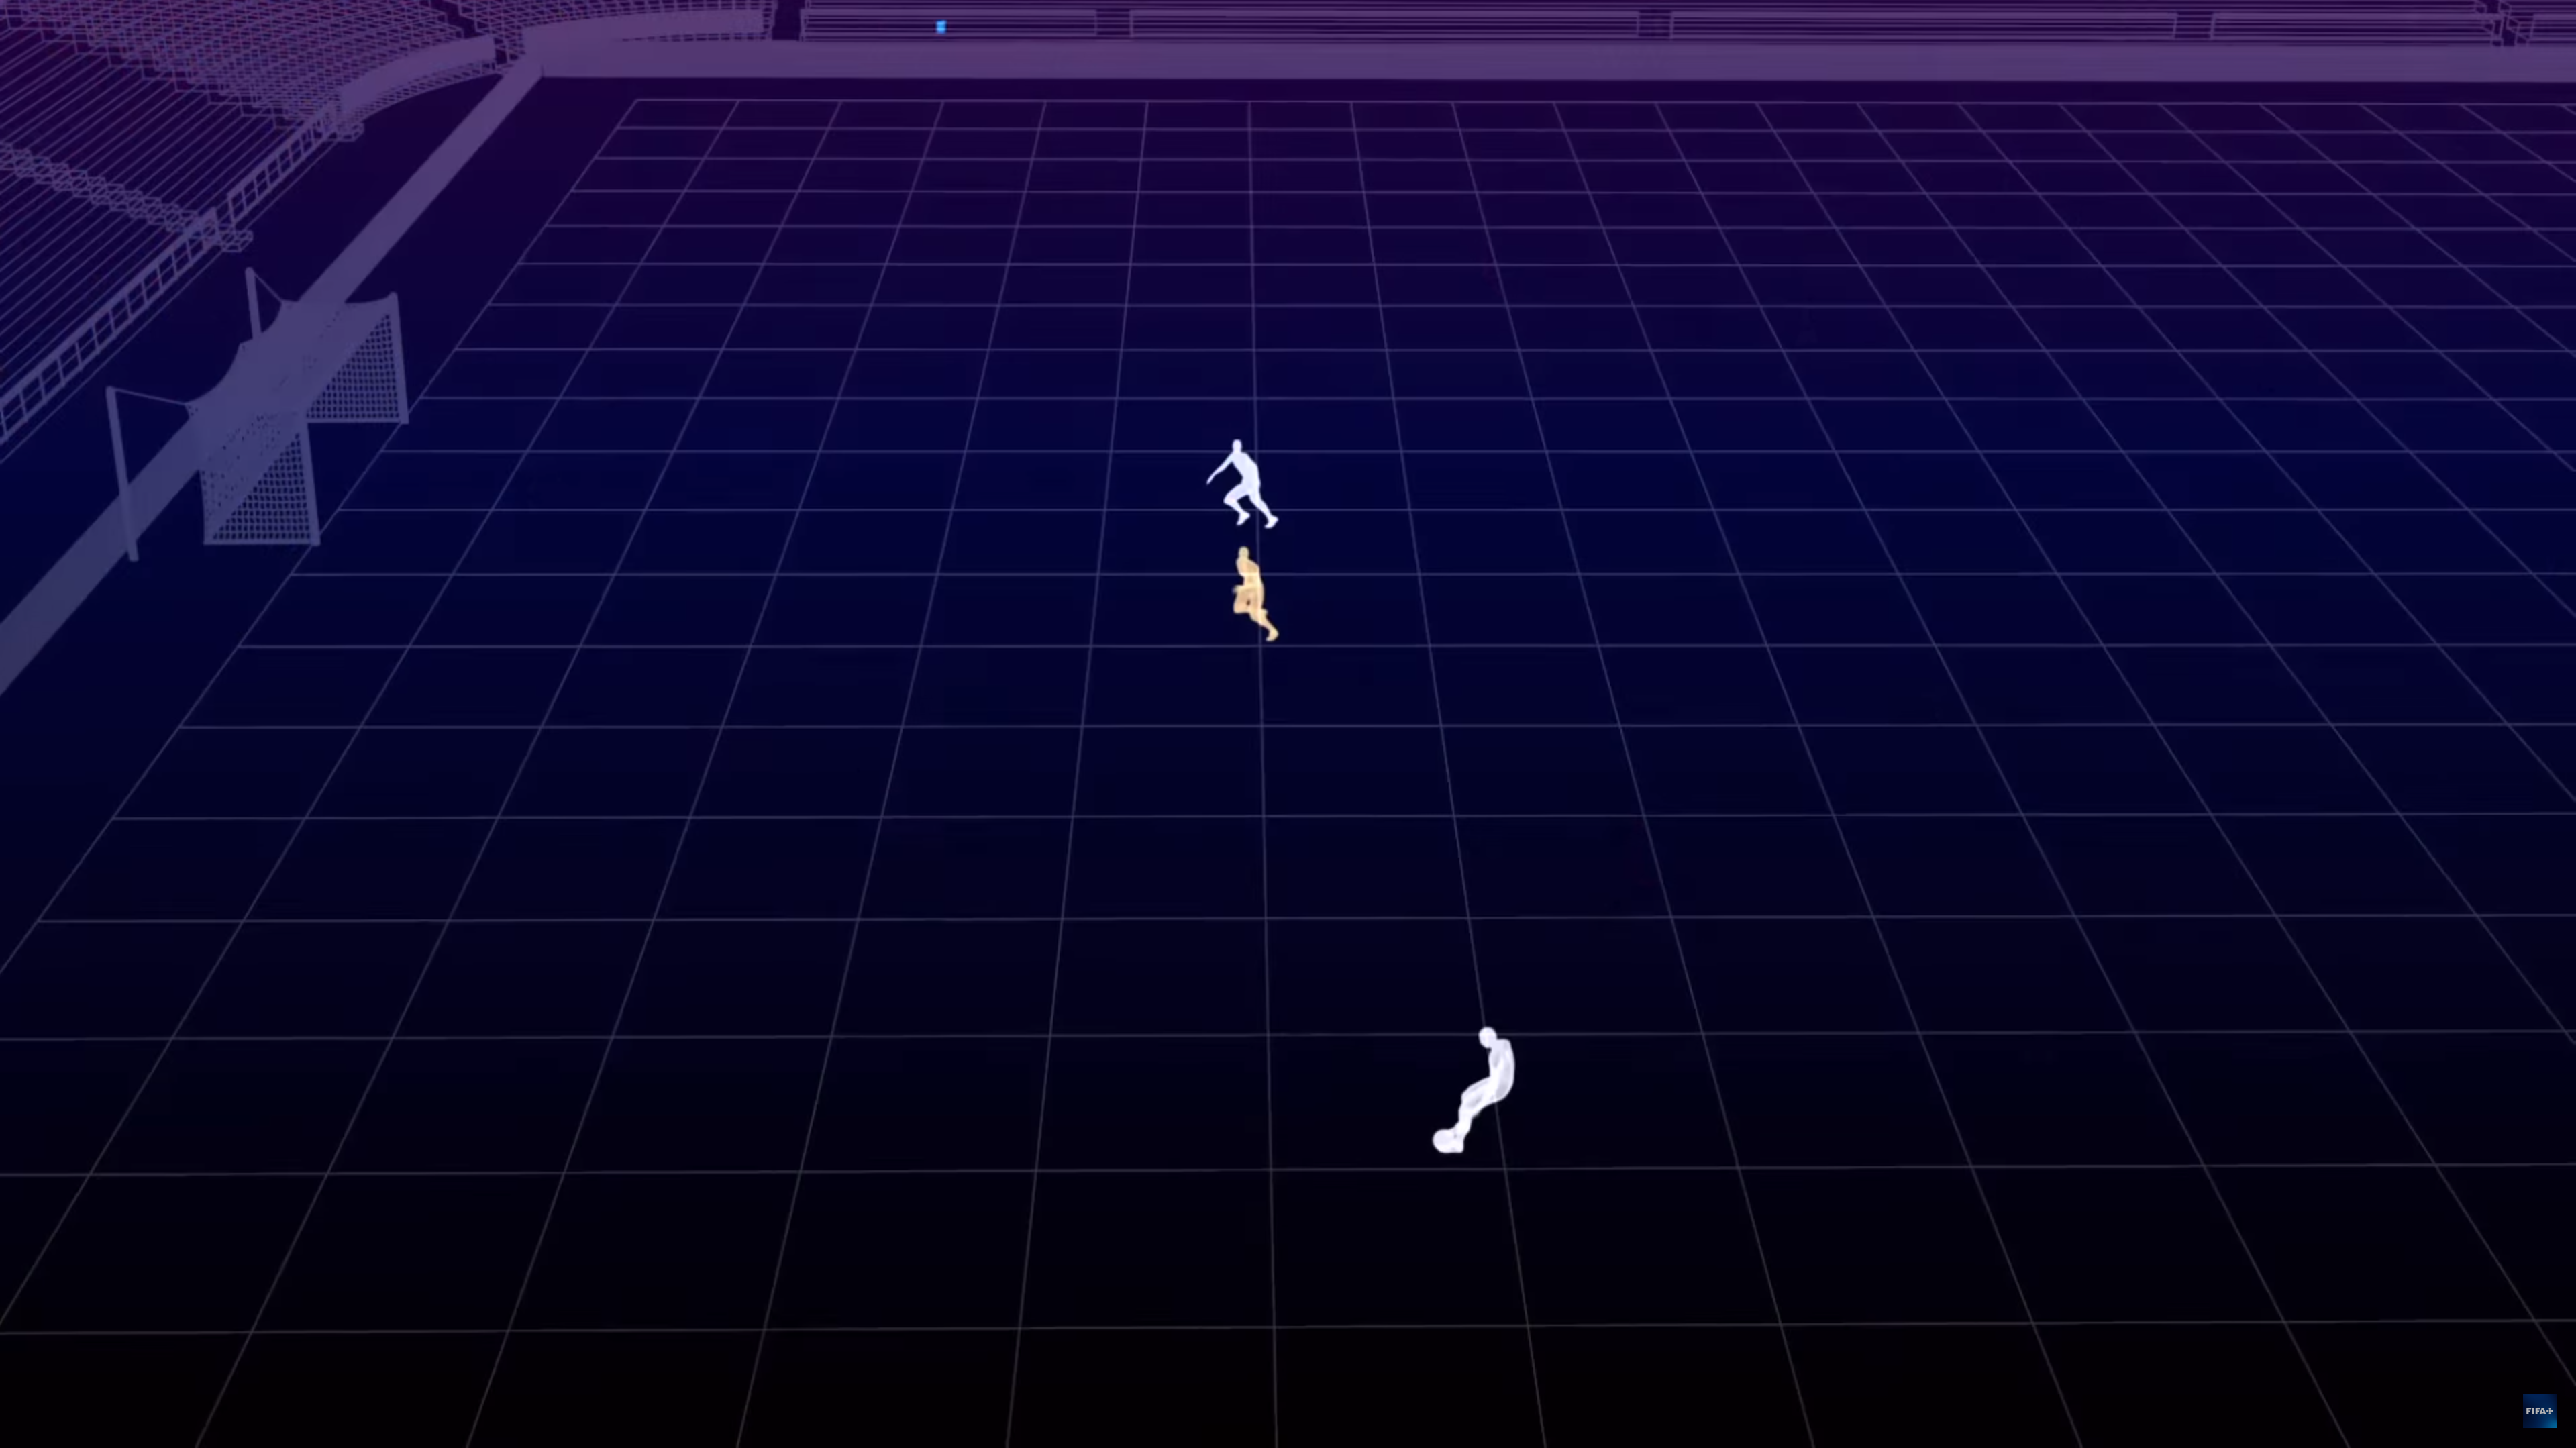
\includegraphics[width=\textwidth]{pic3.png}
		\end{subfigure}
		\begin{subfigure}[b]{0.71\textwidth}
			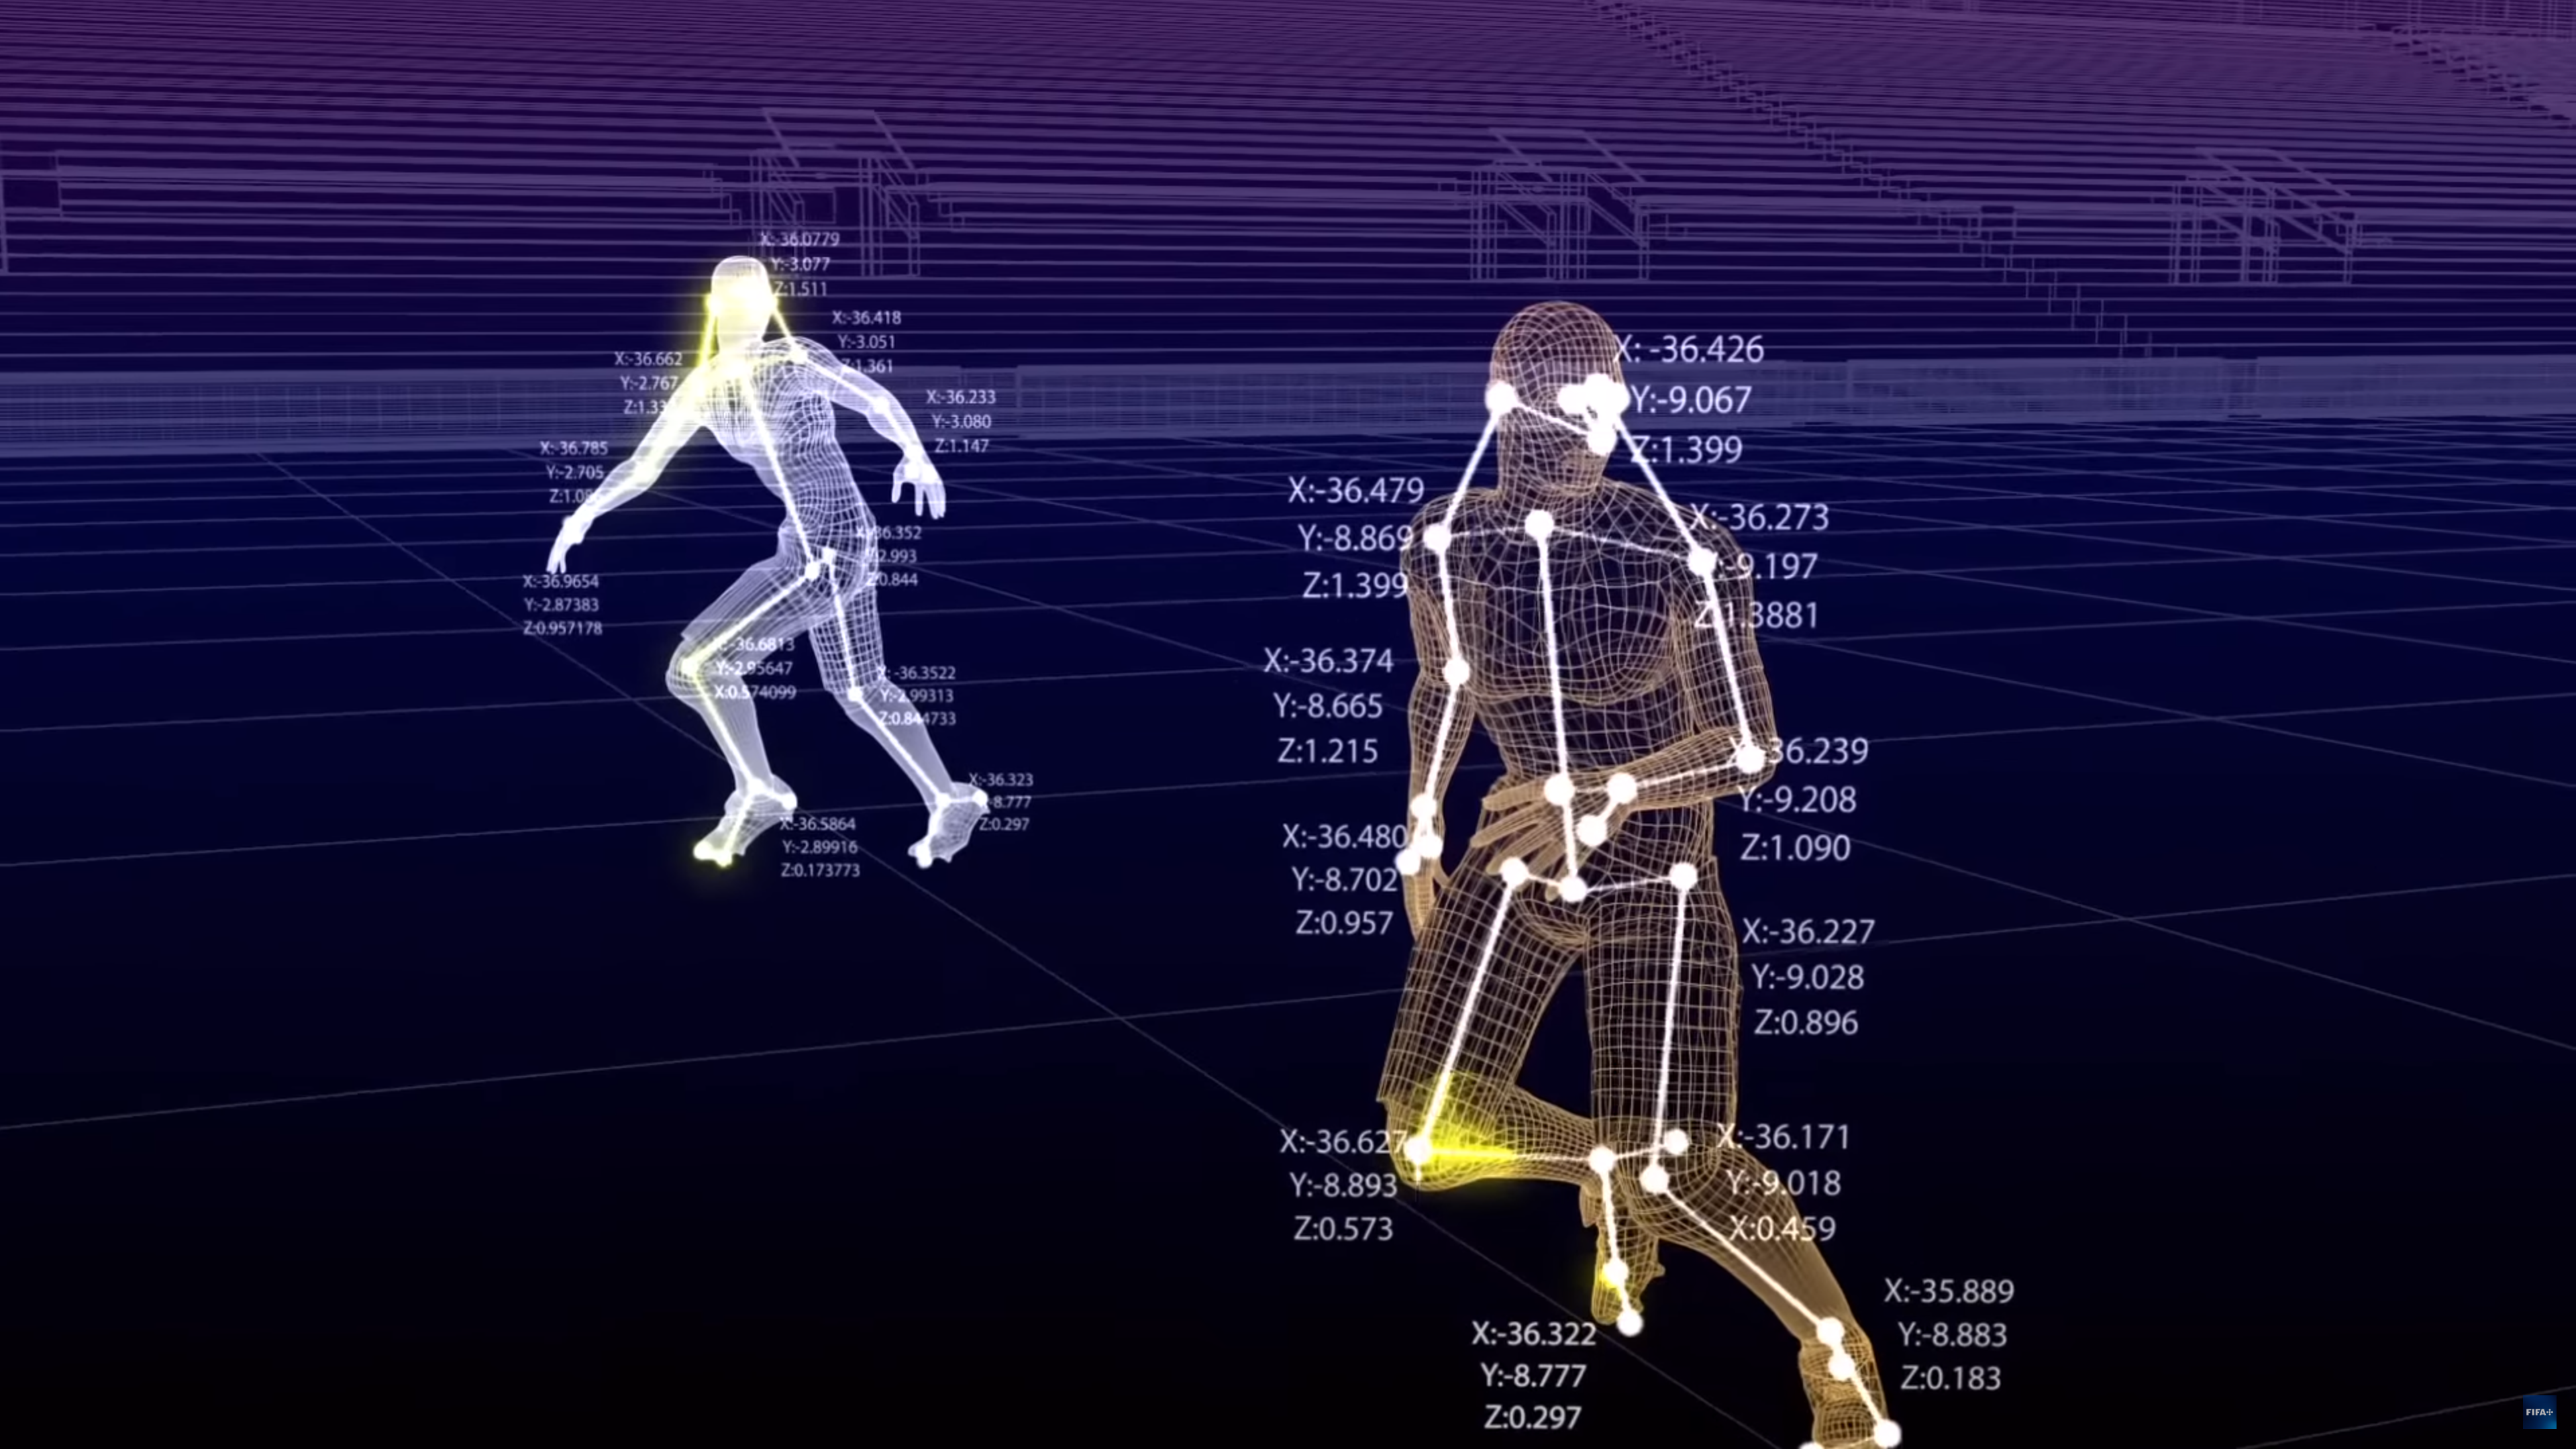
\includegraphics[width=\textwidth]{pic4.png}
		\end{subfigure}
		
		\caption{FIFA Semi Automated Offside Technology Animation\cite{fifa}}
	\end{figure}

	\section{Barriers}
	\subsection{Motion Tracking}
		The environment of the football field is very complex, with similar background interference, changes in lighting conditions, external factors such as occlusion, and changes in target posture.
	\subsection{3D reconstruction}
		According to FIFA official statement, there is a 500Hz sensor inside the football, after obtaining the frame of a pass, reconstruct the 3D position of the player's limbs on the field.
	\subsection{Show to the audience}
		After completing the 3D reconstruction, generate an animation or a picture to tell the audience how the player is offside (if offside).\\
		The images below is an example, by top or side view, or by drawing an offside wall, to show if a player was offside.
	\begin{figure}[ht!]
		\centering
		\begin{subfigure}[b]{0.4\textwidth}
			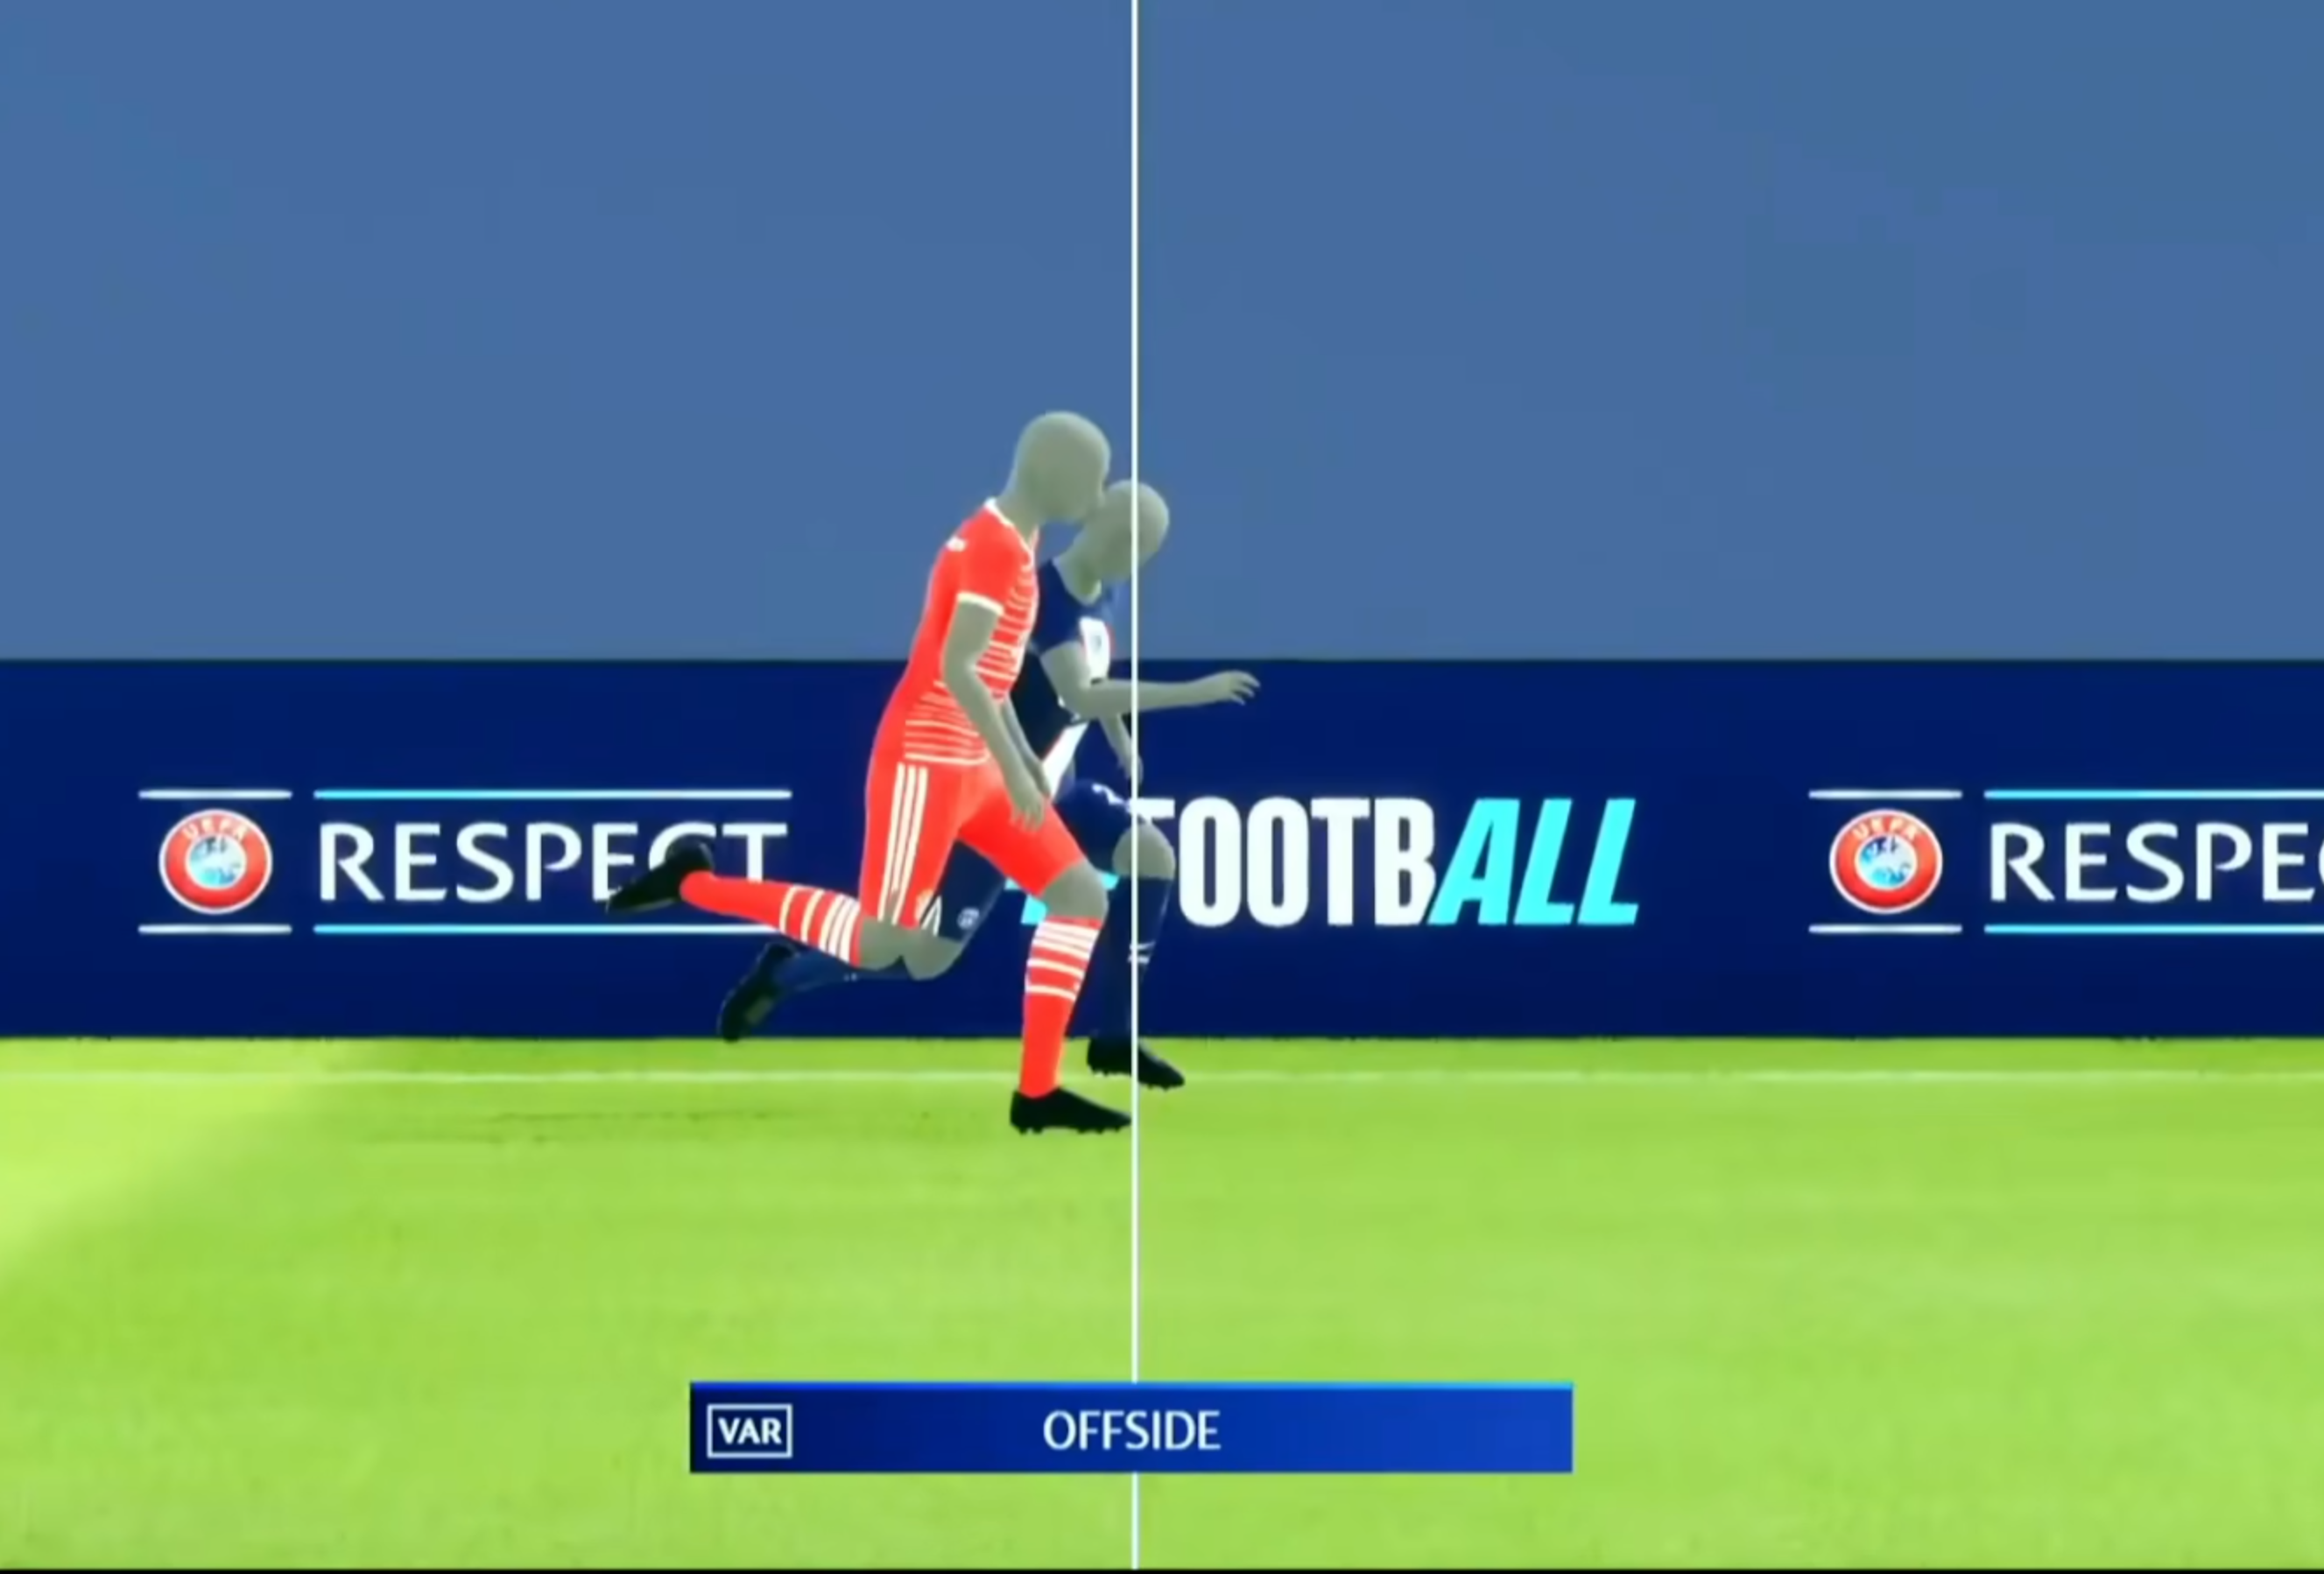
\includegraphics[width=\textwidth]{pic0.png}
		\end{subfigure}
		\begin{subfigure}[b]{0.4\textwidth}
			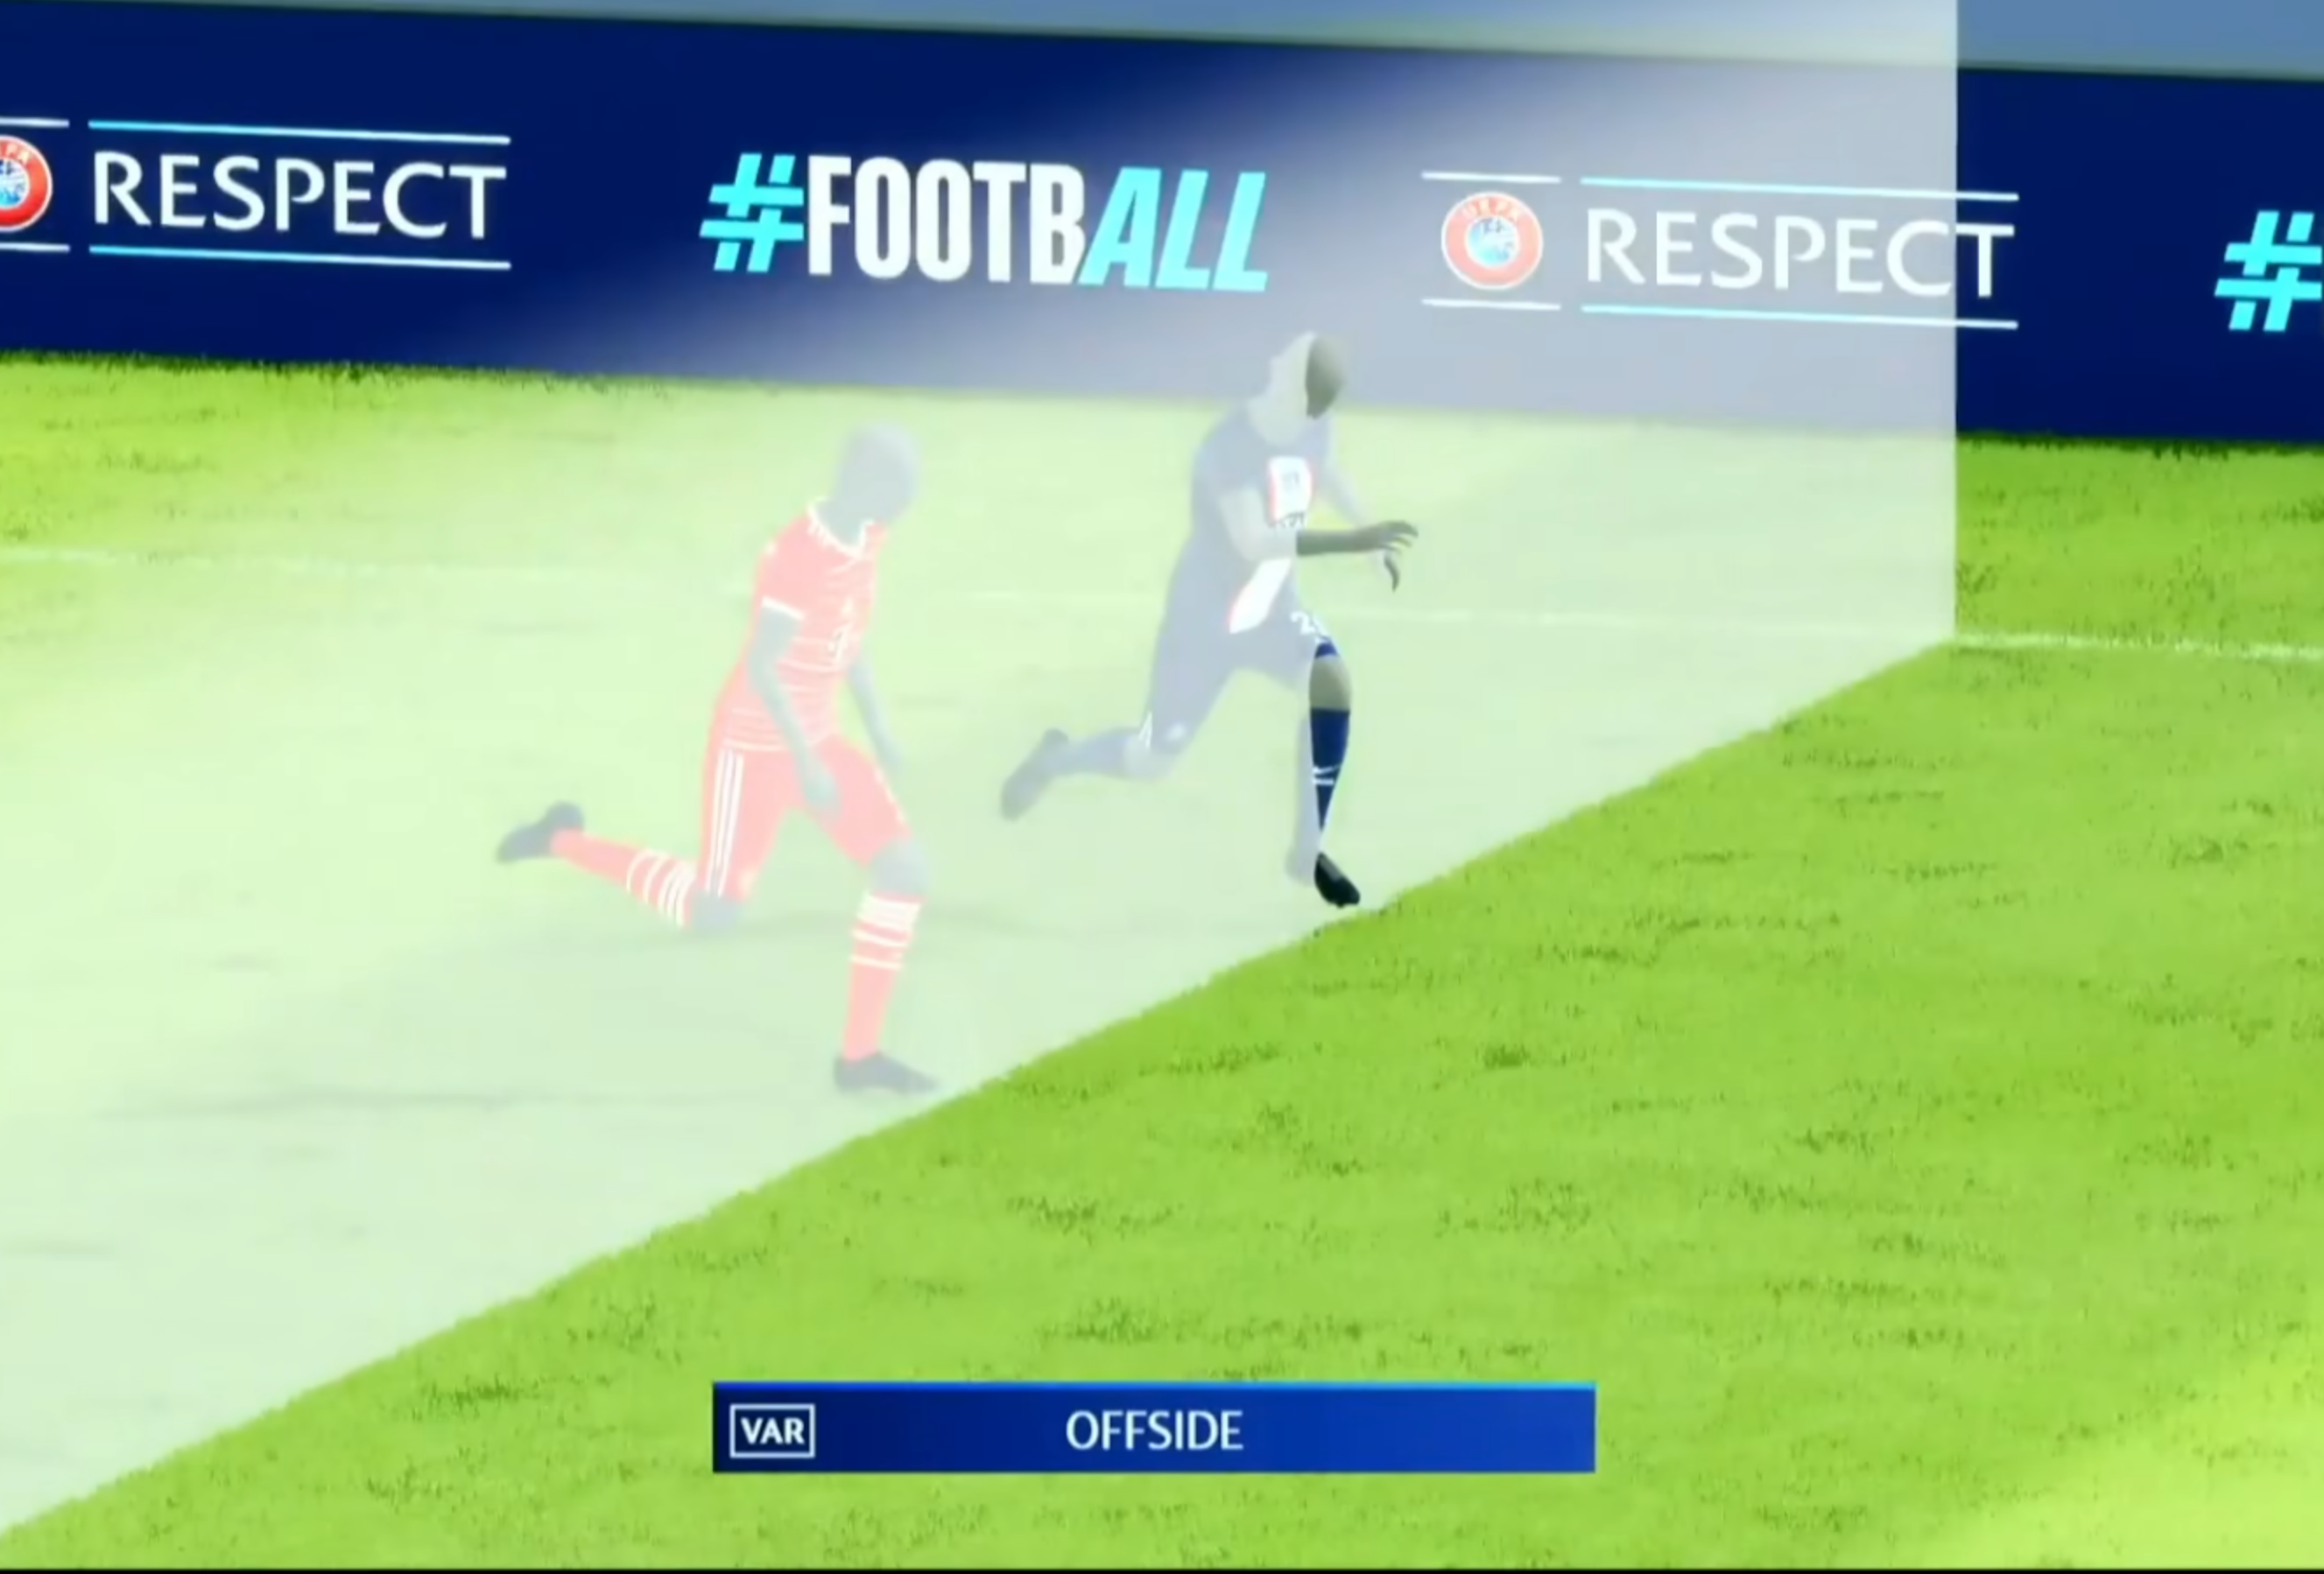
\includegraphics[width=\textwidth]{pic1.png}
		\end{subfigure}
	
		\caption{UCL round of 16 Paris v.s. Bayern 14 Feb 2023\cite{ucl}}
	\end{figure}

	\section{Implementation}
	3D reconstruction is one of the topics of this course, I implemented a very simple model with what I learned in class.\\
	A simple scenario: Suppose the following is the moment of a pass, the white line is the offside line, want to know if my foot crossed the line.
	\begin{figure}[ht!]
		\centering
		\begin{subfigure}[b]{0.4\textwidth}
			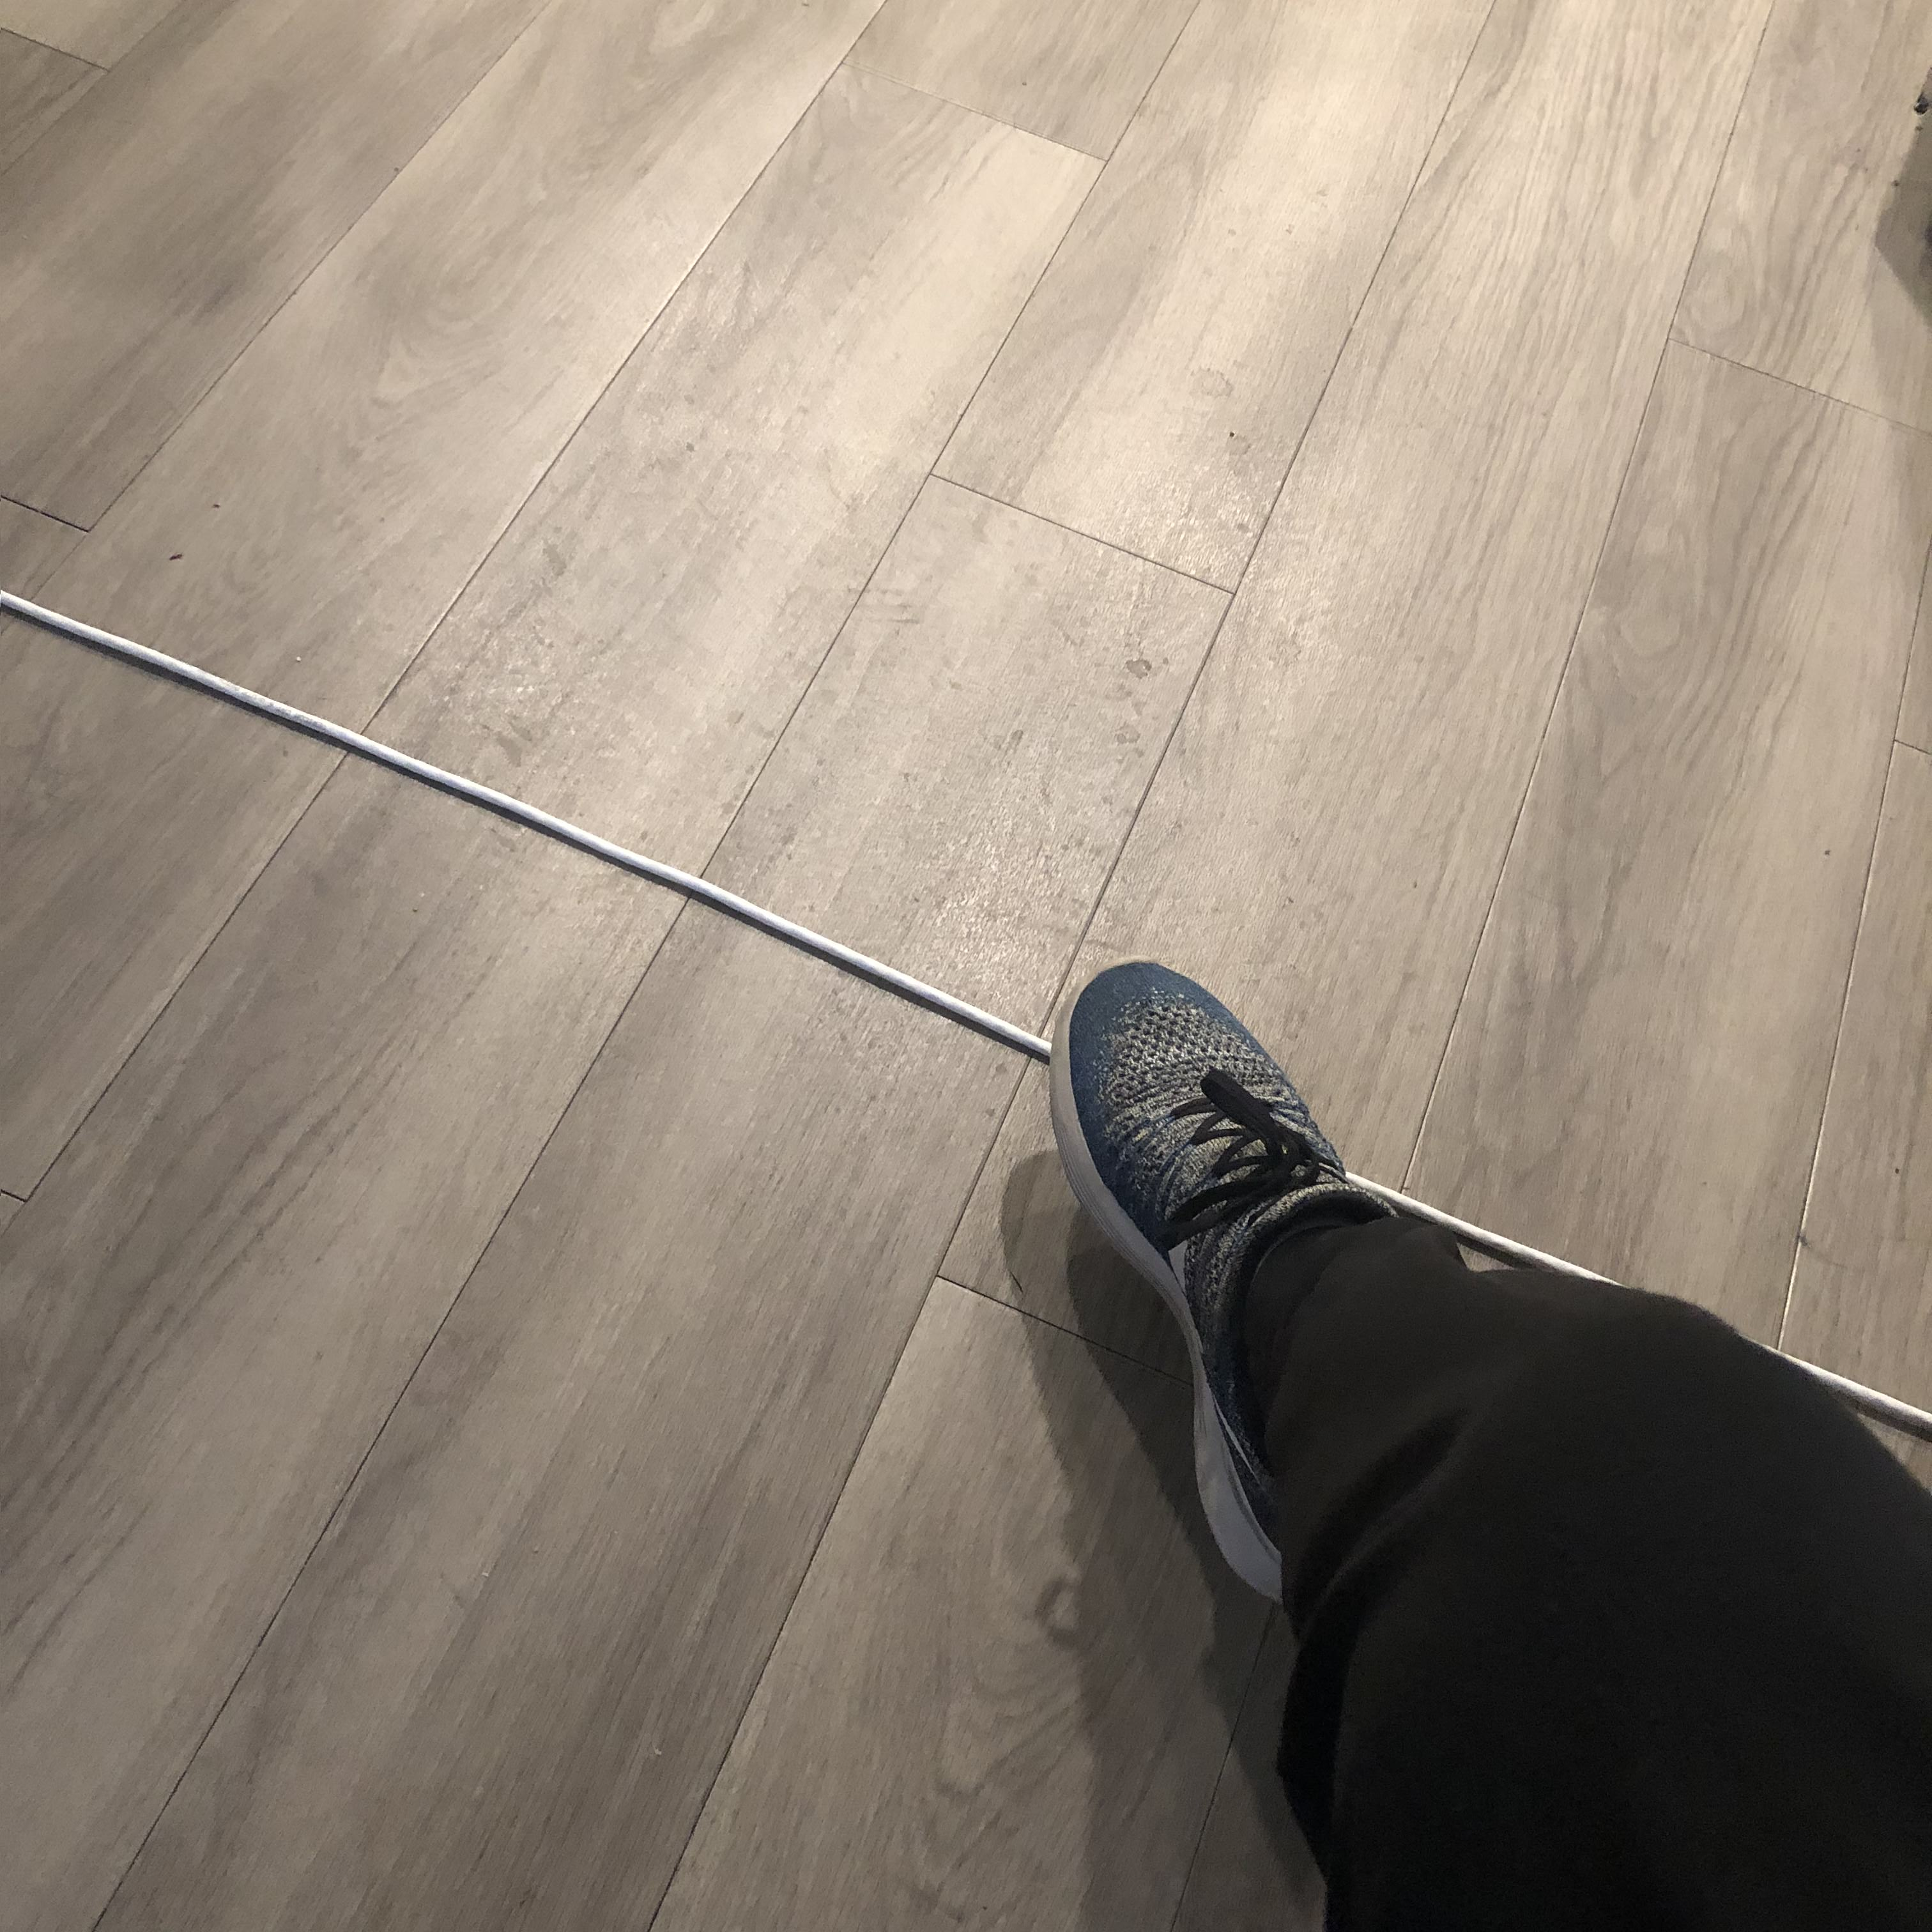
\includegraphics[width=\textwidth]{pic5.jpg}
		\end{subfigure}
		\begin{subfigure}[b]{0.4\textwidth}
			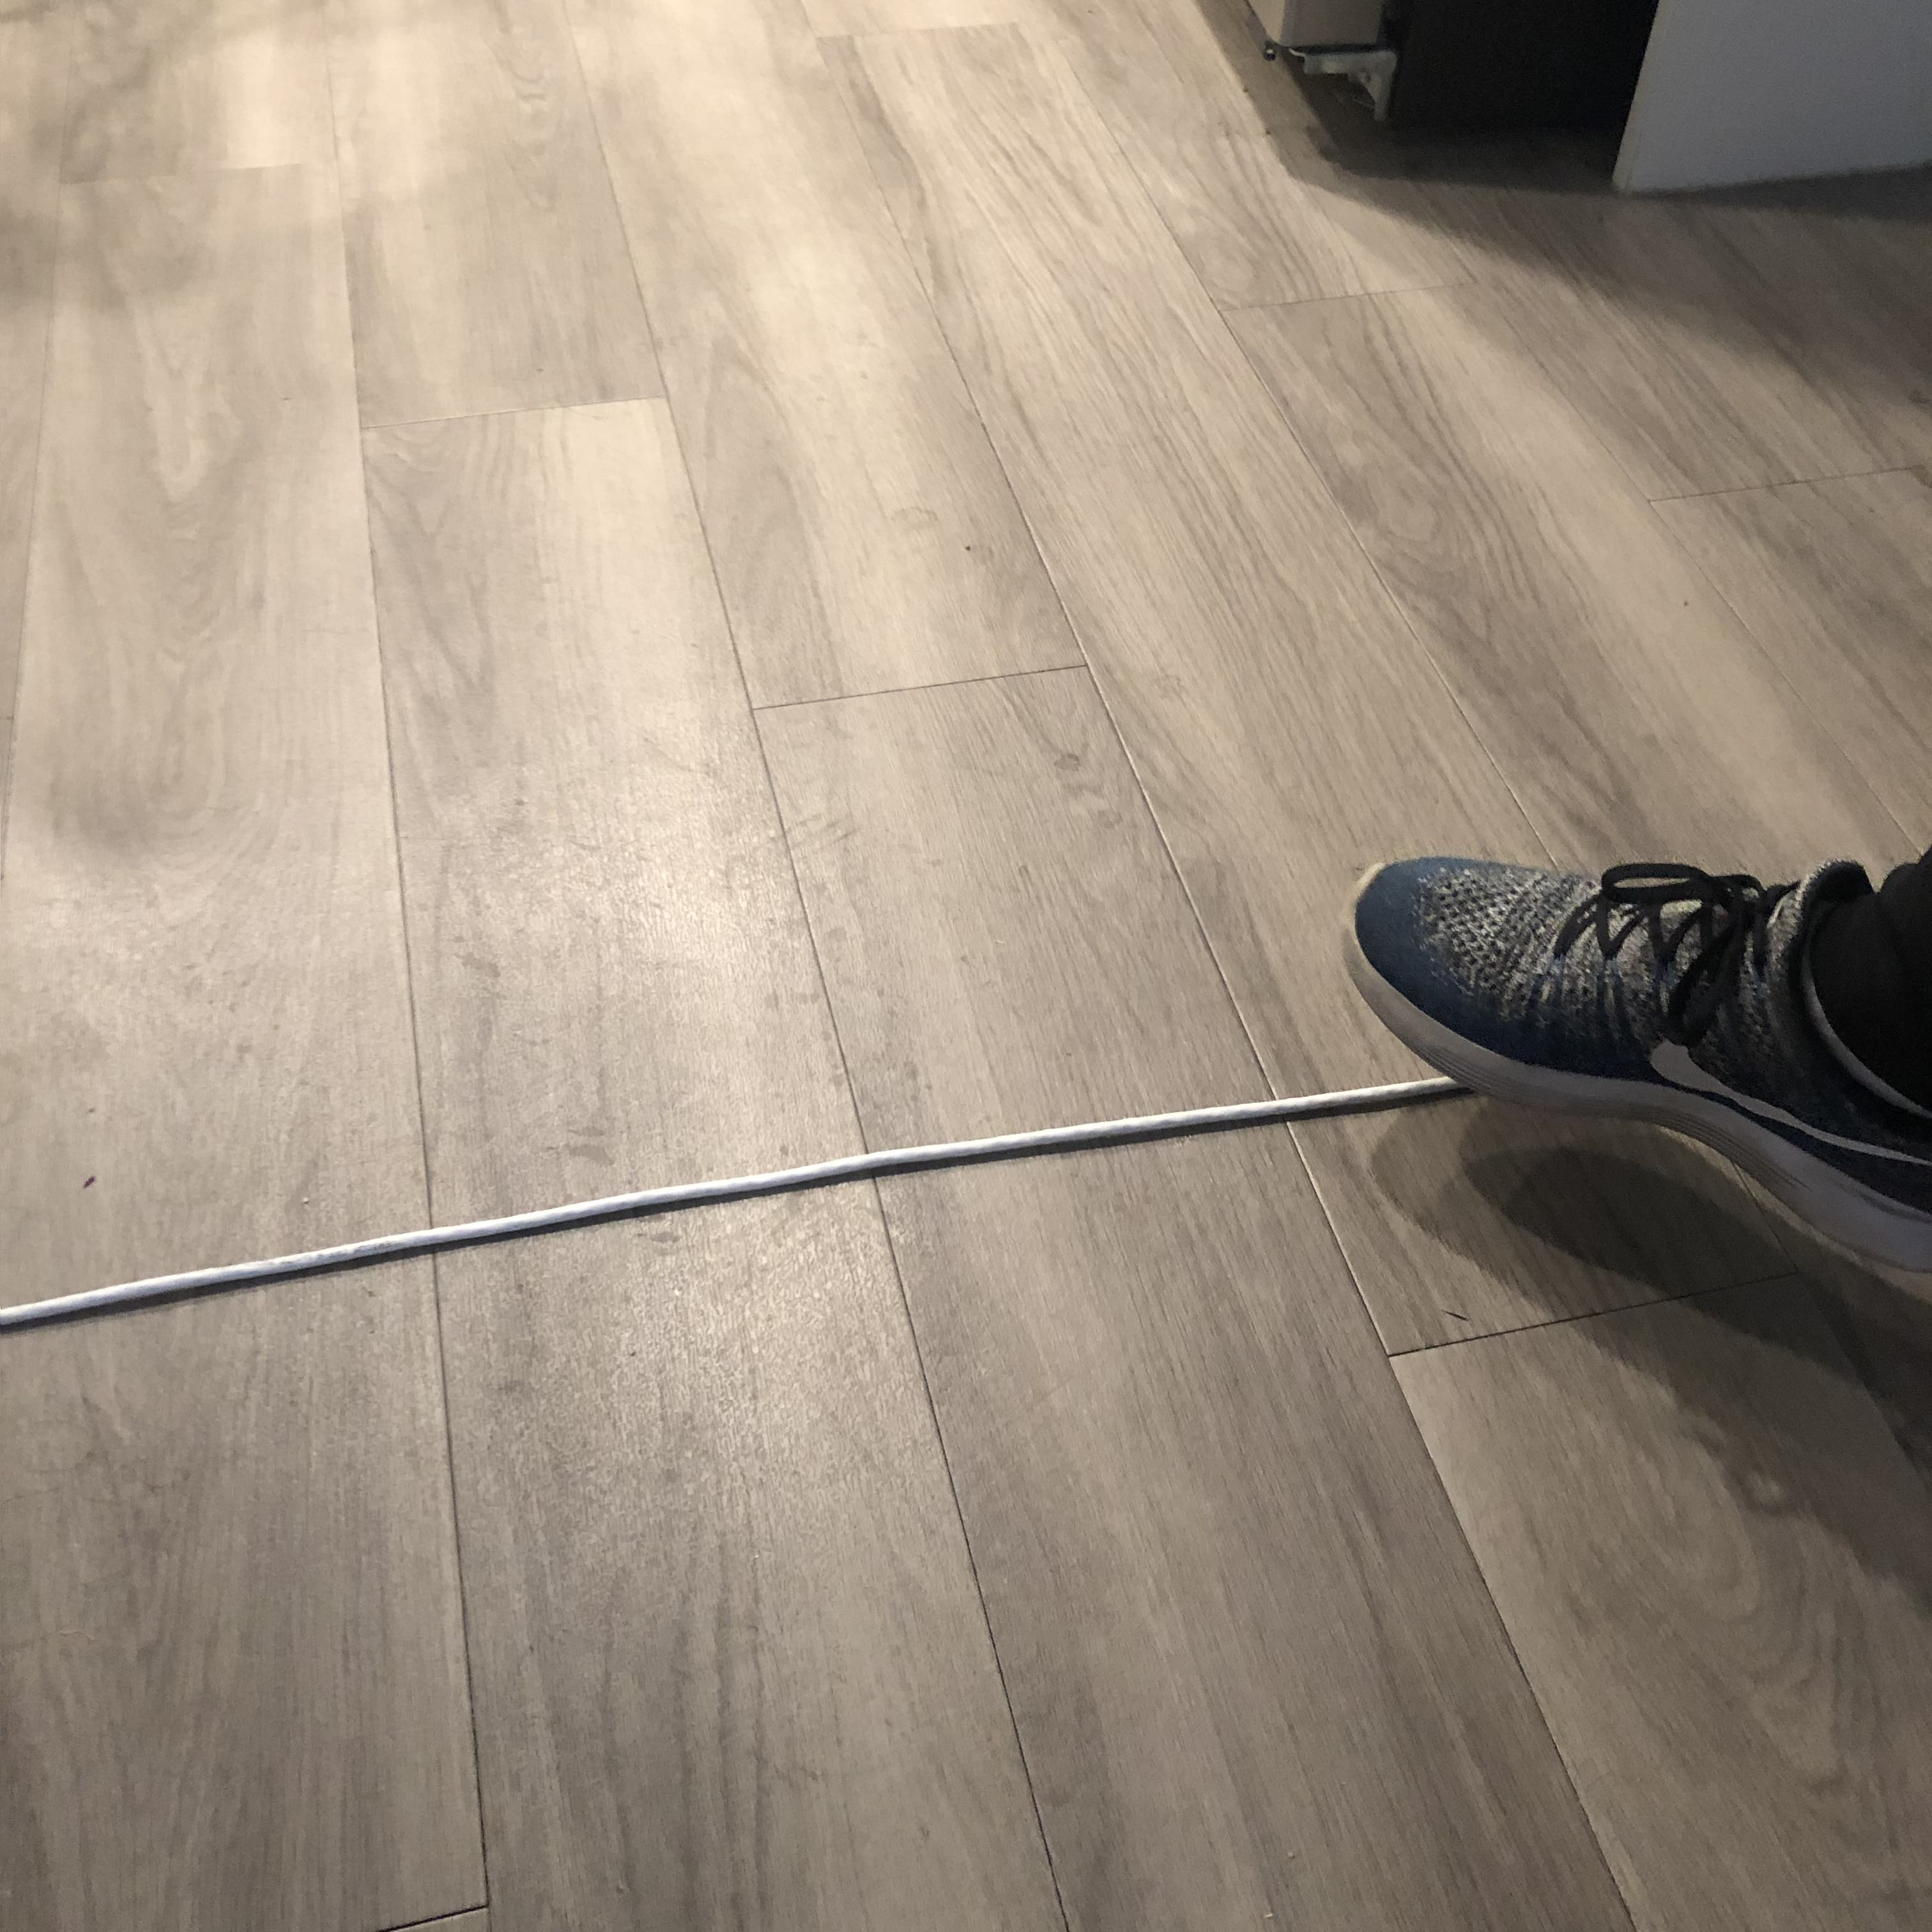
\includegraphics[width=\textwidth]{pic6.jpg}
		\end{subfigure}
		
		\caption{Two views}
	\end{figure}
	
	\subsection{Camera calibration}
		There are many libraries and software to achieve camera calibration. But in order to simplify the problem, I measured the world coordinate system of some points and calculated the focal length, and assumed that there is no skew and distortion.\\
		The approximate Extrinsics are then calculated by least squares.
	\subsection{Find pairs and 3D reconstruction}
		Use the Harris Corner detector to find some corners (the points on the floor are manually added).
		\begin{center}
			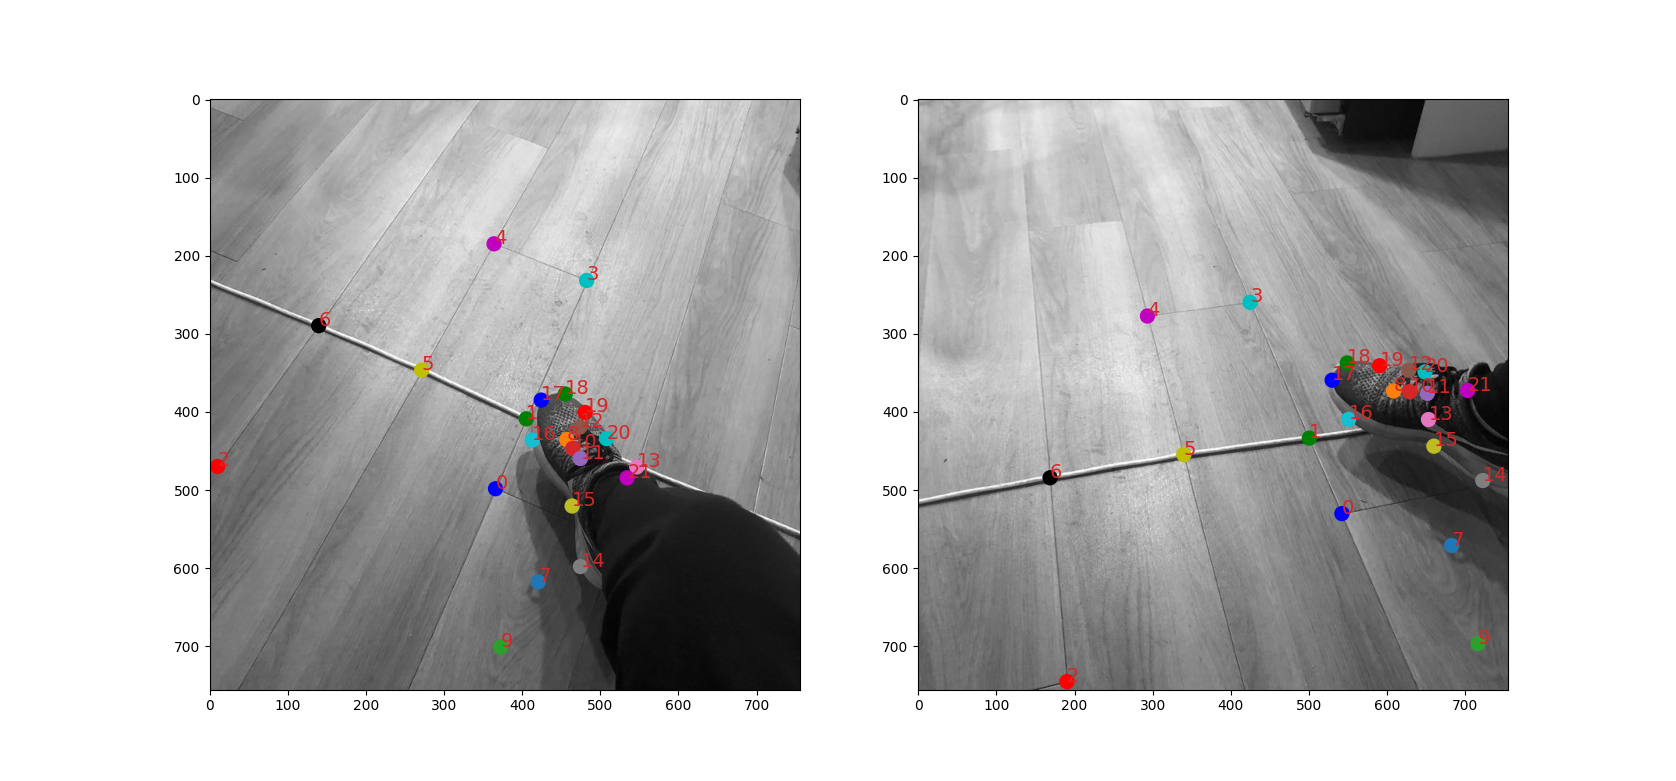
\includegraphics[width=1\textwidth]{points.png}
		\end{center}
		\begin{figure}[ht!]
			\centering
			\begin{subfigure}[b]{0.4\textwidth}
				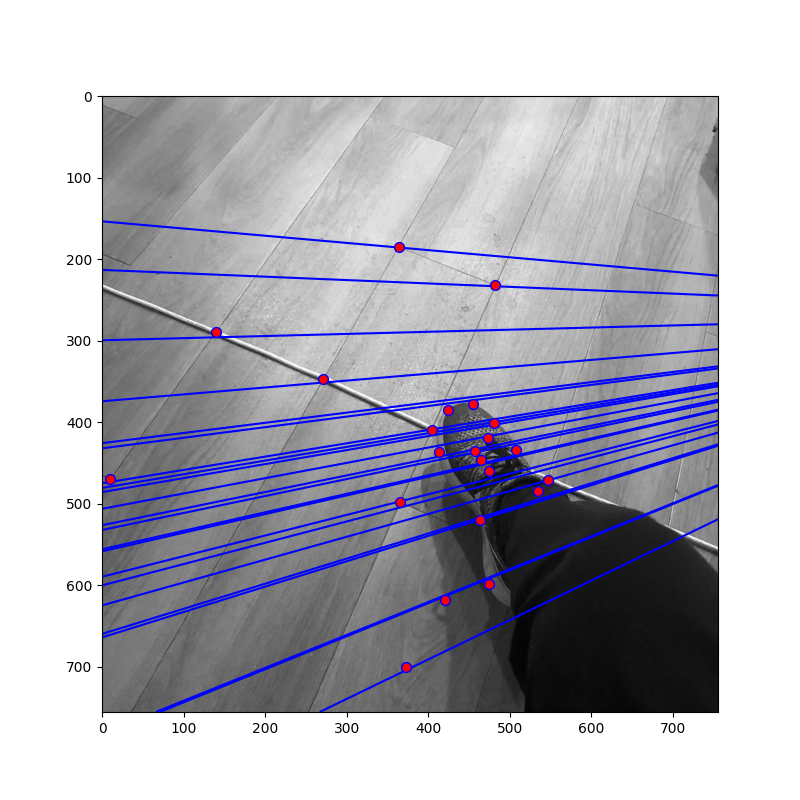
\includegraphics[width=\textwidth]{line1.png}
			\end{subfigure}
			\begin{subfigure}[b]{0.4\textwidth}
				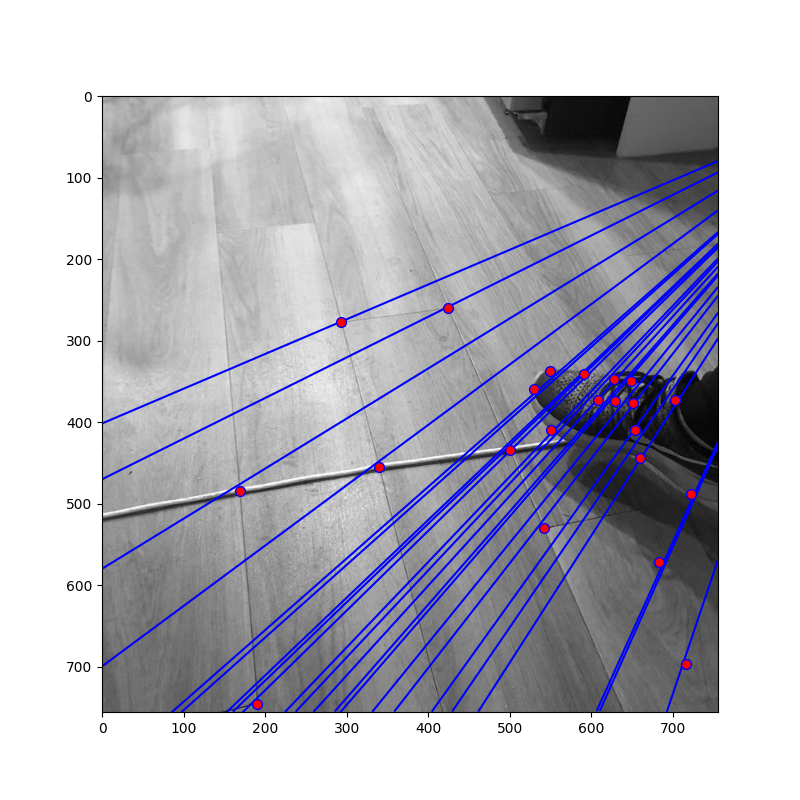
\includegraphics[width=\textwidth]{line2.png}
			\end{subfigure}
			
			\caption{Epipolar lines}
		\end{figure}
	\subsection{Hypothetical camera}
		After obtaining the 3D points, construct a hypothetical camera to obtain a top view. For convenience, the coordinate system of the hypothetical camera is the same as the world coordinate system, that is the z-axis points directly upward. Some points of interest are projected onto this hypothetical camera by projection (the points are added manually to represent the offside line and the outline of the shoe)
		\begin{center}
			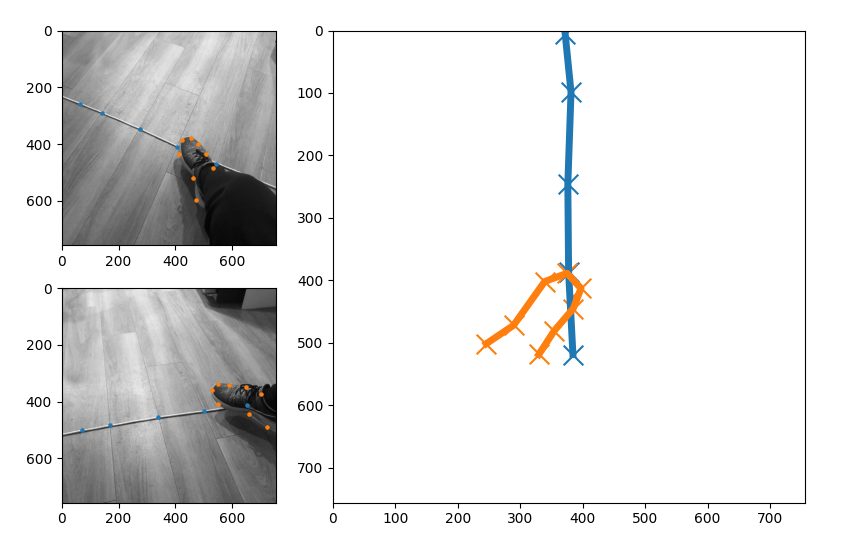
\includegraphics[width=0.75\textwidth]{results.png}
		\end{center}
		Despite its poor accuracy, the model does convert two difficult-to-see offside images into an easy-to-see projection.\\
		\href{mailto:claudio.vellage@latex-tutorial.com}{claudio.vellage@latex-tutorial.com}
	\newpage
	\bibliographystyle{apalike}
	\bibliography{reference}
\end{document}